\documentclass{beamer}
\usetheme{Gelugor}
\usepackage{hyperref}
\usepackage[utf8]{inputenc}
\usepackage[spanish]{babel}
\usepackage[default]{droidserif}
\title{Análisis y Diseño de Software}
\subtitle{Práctica}
\author[Grupo1]{
Martha Suntaxi\\Johanna Paz\\Victor Jumbo\\Andre Montoya\\Wilson Iriarte
}
\date{\today}
\institute{Ingeniería en Sistemas\\}

\begin{document}
	
	%INICIO carátula
	\begin{frame}[plain,t]
		\titlepage
	\end{frame}
	%FIN carátula

	\section{Práctica}

\subsection{Agenda}
\begin{frame}
\frametitle{Agenda}
{\small
\begin{enumerate}
	\item Instalacion de github
	\item Configuración
	\item Vinculación
	\item Repositorios github
\end{enumerate}
}
\end{frame}
\subsection{Instalacion de gitguh}
		\begin{frame}
			\frametitle{Instalacion de github}
			%\framesubtitle{Tema}
			1. Para Linux, mediante el siguiente comando:\\
			{\tt \scriptsize sudo apt-get install git-core}\\
			\begin{center}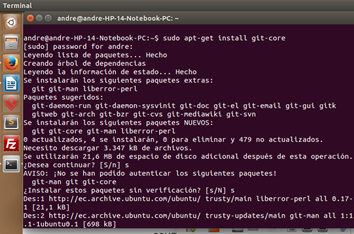
\includegraphics[width=5cm, height=3cm]{1.png}\end{center}
		\end{frame}
		
\subsection{Configuración}
	\begin{frame}
			\frametitle{Configuración}
			%\framesubtitle{Tema}
			2. Una vez instalado Github, procedemos a configurarlo; para ello debemos configurar primero el 								nombre de usuario haciendo uso del siguiente comando:\\
			\begin{center}
				 {\tt \scriptsize git config --global user.name User Name}\\
			\end{center}
			\begin{center}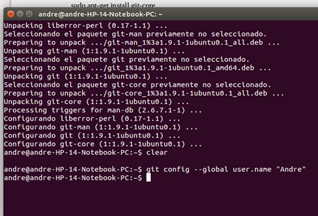
\includegraphics[width=5cm, height=3cm]{2.png}\end{center}
	\end{frame}
		
	\begin{frame}
			\frametitle{Configuración}
			%\framesubtitle{Tema}
			Una vez configurado el nombre de usuario, procedemos a configurar el email del usuario, haciendo 						uso del siguiente comando:\\
			\begin{center}
				 {\tt \scriptsize git config --global user.email tuemail@dominio.com}\\
			\end{center}
			\begin{center}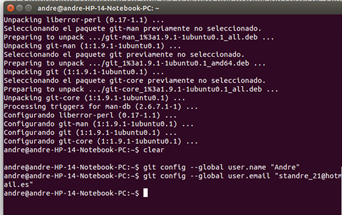
\includegraphics[width=5cm, height=3cm]{3.png}\end{center}
	\end{frame}

\subsection{Vinculación}
	\begin{frame}
		\frametitle{Vinculación}
		{\small 3. Luego de haber configurado github, procedemos a vincular nuestra pc con github. Para ello generaremos una SSH KEY que posteriormente registraremos en nuestra cuenta de github haciendo uso del siguiente comando:}
		\begin{center}
			 {\tt \scriptsize ssh-keygen -t rsa -C tuemail@dominio.com}\\
		\end{center}
		{\small una vez ingresado el comando nos pedira que ingresemos un nombre cualquiera en este casi fue key.txt para el archivo donde se guardara la SSH KEY:}
		\begin{center}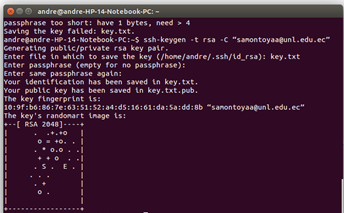
\includegraphics[width=5cm, height=3cm]{4.png}\end{center}
	\end{frame}
	
	\begin{frame}
		\frametitle{Vinculación}
		4. Una vez generada la SSH KEY nos dirigimos al dirctorio home y visualizaremos el archivo con el nombre que le dimos, en este fue key.txt
		\begin{center}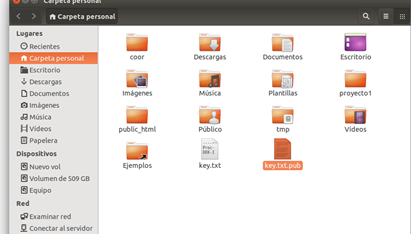
\includegraphics[width=8cm, height=5cm]{5.png}\end{center}
	\end{frame}
	\begin{frame}
		\frametitle{Vinculación}
		{\small 5. Abrimos este archivo copiamos el contenido, nos dirigimos anuestra cuenta de github en la pestaña de configuraciones visualizaremos SSH KEY y pegamos el contenido antes menciondo:}
		\begin{center}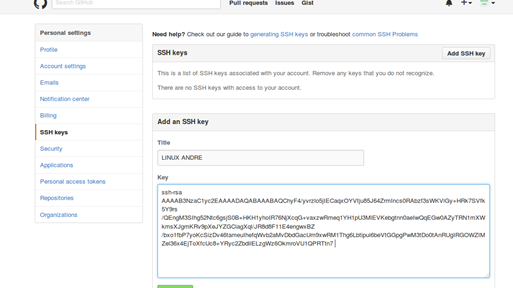
\includegraphics[width=8cm, height=5cm]{6.png}\end{center}
	\end{frame}

\subsection{Repositorios gitguh}
	\begin{frame}
		\frametitle{Repositorios github}
		{\small 6. Una vez vinculada nuestra pc con github, podemos empezar a trabajar con repositorios github. Para ello creamos un repositorio nuevo desde la web de github:}
		\begin{center}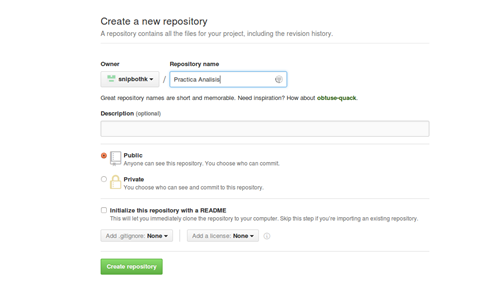
\includegraphics[width=8cm, height=5cm]{7.png}\end{center}
	\end{frame}
	
	\begin{frame}
		\frametitle{Repositorios github}
		{\small 7. Luego creamos una carpeta en nuestro directorio personal, donde se almacenaran nuestros repositorios github:}
		\begin{center}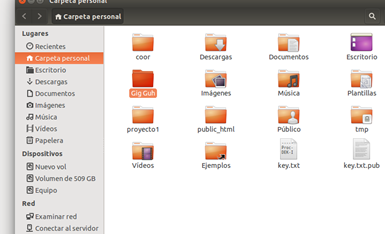
\includegraphics[width=8cm, height=5cm]{8.png}\end{center}
	\end{frame}
	
	\begin{frame}
		\frametitle{Repositorios github}
		{\small 8. En consola escribimos el siguiente comando:}
		\begin{center}
			 {\tt \scriptsize cd /home/Nombre de la carpeta}\\
		\end{center}
		{\small En este caso sería:}
		\begin{center}
			 {\tt \scriptsize cd /home/GitHub}\\
		\end{center}
	\end{frame}
	
	\begin{frame}
		\frametitle{Repositorios github}
		{\small 9. Una ves dentro de la carpeta escribimos los comandos en el siguiente orden:}\\
			 {\tt \scriptsize echo "\# Practica-Analisis” >> README.md}\\
			 {\tt \scriptsize git init}\\
			 {\tt \scriptsize git add README.md}\\
			 {\tt \scriptsize git commit -m "first commit”}\\
			 {\tt \scriptsize git remote add origin git@github.com:snipbothk/Practica-Analisis.git}\\
			 {\tt \scriptsize git push -u origin master}\\
		{\small Reemplazamos “Practica Analisis”por el nombre de su repositorio., y “snipbothk/Practica-Analisis.git” por su usuario github y el nombre de su repositorio, quedando “User/Mirepositorio.git”.}
	\end{frame}
	
	\begin{frame}
		\frametitle{Repositorios gitguh}
		{\small 10. Luego de esto podemos verificar en nuestra cuenta de GitHub dentro del repositorio que creamos, como nuestro fichero README.md se ha añadido correctamente:}
		\begin{center}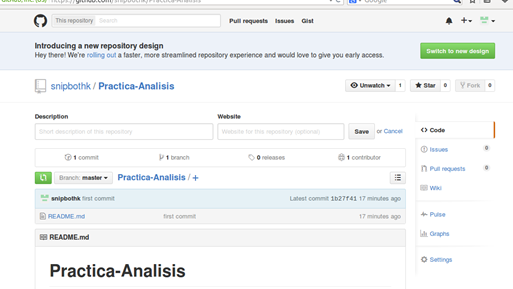
\includegraphics[width=8cm, height=5cm]{10.png}\end{center}
	\end{frame}
	
\subsection{Bibliografía}
\begin{frame}
\frametitle{Bibliografia}
	\begin{enumerate}
		\item L. Castillo, Conociendo GitHub. \url{https://conociendogithub.readthedocs.org/en/latest/}.
		\item J. Soto, Mi Primer Libro.  Concepción, Chile: McGraw-Hill, 2013.
	\end{enumerate}
\end{frame}

\subsection{Licencia}
\begin{frame}
\frametitle{Licencia}
\begin{center}
\href{http://www.google.com}{
\includegraphics[scale=.8]{cc}}
\end{center}
\end{frame}

\MuchasGraciasFrame

\end{document}
